\documentclass[tikz,border=6pt]{standalone}
\usepackage[T1]{fontenc}
\usepackage{lmodern}
\usepackage{amsmath,amssymb}
\usepackage{tikz}
\usetikzlibrary{positioning,arrows.meta,calc}

\tikzset{
  >={Stealth[length=1.9mm]},
  st/.style={circle,draw,thick,minimum size=7.2mm,inner sep=0pt,font=\small},
  ab/.style={circle,draw,thick,double,double distance=0.7pt,
             minimum size=7.2mm,inner sep=0pt,font=\small},
  lb/.style={font=\footnotesize,inner sep=1.4pt},
  note/.style={font=\small\itshape,text=black!70},
  paneltitle/.style={font=\small\bfseries},
  every path/.style={thick}
}

\begin{document}
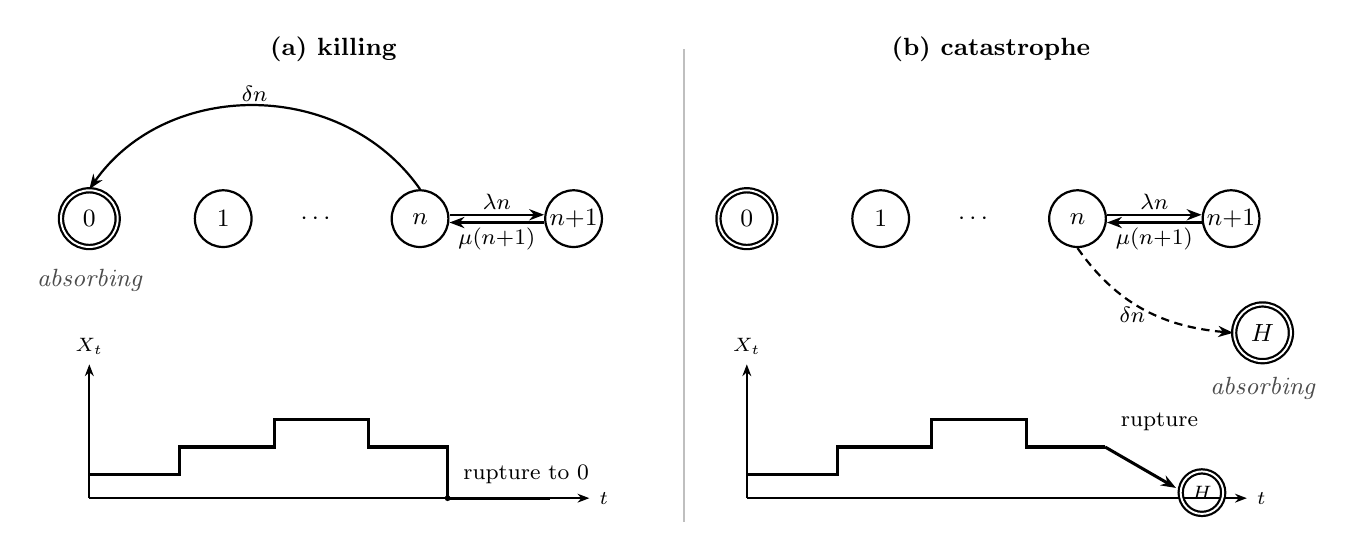
\begin{tikzpicture}[font=\small]
  % ---- killing ----
  \begin{scope}
    \node[paneltitle] at (3.1,2.15) {(a) killing};
    \node[ab] (k0) at (0,0) {$0$};
    \node[st] (k1) at (1.7,0) {$1$};
    \node at (2.9,0) {$\cdots$};
    \node[st] (kn) at (4.2,0) {$n$};
    \node[st] (knp) at (6.15,0) {$n{+}1$};
    \draw[->] ([yshift=1.4pt]kn.east) -- node[above,lb]{$\lambda n$} ([yshift=1.4pt]knp.west);
    \draw[->] ([yshift=-1.4pt]knp.west) -- node[below,lb]{$\mu(n{+}1)$} ([yshift=-1.4pt]kn.east);
    \draw[->] (kn.north) to[out=125,in=55,looseness=1.05]
      node[above,lb]{$\delta n$} (k0.north);
    \node[note] at (0,-0.78) {absorbing};

    \draw[-{Stealth[length=1.5mm]},line width=0.7pt] (0,-3.55) -- (6.35,-3.55)
      node[right,font=\scriptsize] {$t$};
    \draw[-{Stealth[length=1.5mm]},line width=0.7pt] (0,-3.55) -- (0,-1.85)
      node[above,font=\scriptsize] {$X_t$};
    \draw[line width=1.1pt]
      (0,-3.25) -- (1.15,-3.25) -- (1.15,-2.90) -- (2.35,-2.90)
      -- (2.35,-2.55) -- (3.55,-2.55) -- (3.55,-2.90) -- (4.55,-2.90)
      -- (4.55,-3.55) -- (5.85,-3.55);
    \fill (4.55,-3.55) circle[radius=1.05pt];
    \node[font=\footnotesize,anchor=south west] at (4.62,-3.50) {rupture to $0$};
  \end{scope}

  % ---- catastrophe ----
  \begin{scope}[shift={(8.35,0)}]
    \node[paneltitle] at (3.1,2.15) {(b) catastrophe};
    \node[ab] (c0) at (0,0) {$0$};
    \node[st] (c1) at (1.7,0) {$1$};
    \node at (2.9,0) {$\cdots$};
    \node[st] (cn) at (4.2,0) {$n$};
    \node[st] (cnp) at (6.15,0) {$n{+}1$};
    \draw[->] ([yshift=1.4pt]cn.east) -- node[above,lb]{$\lambda n$} ([yshift=1.4pt]cnp.west);
    \draw[->] ([yshift=-1.4pt]cnp.west) -- node[below,lb]{$\mu(n{+}1)$} ([yshift=-1.4pt]cn.east);
    \node[ab] (cH) at (6.55,-1.45) {$H$};
    \draw[->,densely dashed] (cn.south) to[out=-55,in=175]
      node[below,lb,pos=0.42]{$\delta n$} (cH.west);
    \node[note] at (6.55,-2.15) {absorbing};

    \draw[-{Stealth[length=1.5mm]},line width=0.7pt] (0,-3.55) -- (6.35,-3.55)
      node[right,font=\scriptsize] {$t$};
    \draw[-{Stealth[length=1.5mm]},line width=0.7pt] (0,-3.55) -- (0,-1.85)
      node[above,font=\scriptsize] {$X_t$};
    \draw[line width=1.1pt]
      (0,-3.25) -- (1.15,-3.25) -- (1.15,-2.90) -- (2.35,-2.90)
      -- (2.35,-2.55) -- (3.55,-2.55) -- (3.55,-2.90) -- (4.55,-2.90);
    \draw[->,line width=1.1pt] (4.55,-2.90) -- (5.45,-3.42);
    \node[ab,minimum size=5.4mm,font=\scriptsize] at (5.78,-3.48) {$H$};
    \node[font=\footnotesize,anchor=south west] at (4.62,-2.82) {rupture};
  \end{scope}

  \draw[black!25,line width=0.6pt] (7.55,2.15) -- (7.55,-3.85);
\end{tikzpicture}
\end{document}
